\documentclass{article}[12pt]
\setlength{\topmargin}{-0.8in}
\setlength{\oddsidemargin}{0in}
\setlength{\textwidth}{6.5in}
\setlength{\textheight}{9.25in}
\usepackage{fullpage, amsmath, amsthm, amssymb,spverbatim, indentfirst,xcolor,fancyvrb}

\usepackage{graphicx}
\usepackage[T1]{fontenc}
\usepackage{mathpazo}
\usepackage{caption}
\usepackage{adjustbox}
\usepackage{enumerate}
\usepackage{geometry}
\usepackage{textcomp}
\usepackage{upquote}
\usepackage{eurosym}
\usepackage[mathletters]{ucs}
\usepackage[utf8x]{inputenc}
\usepackage{grffile}
\usepackage{hyperref}
\usepackage{longtable}
\usepackage{booktabs}
\usepackage[inline]{enumitem}
\usepackage[normalem]{ulem}

% Colors for the hyperref package
    \definecolor{urlcolor}{rgb}{0,.145,.698}
    \definecolor{linkcolor}{rgb}{.71,0.21,0.01}
    \definecolor{citecolor}{rgb}{.12,.54,.11}
    
        % ANSI colors
    \definecolor{ansi-black}{HTML}{3E424D}
    \definecolor{ansi-black-intense}{HTML}{282C36}
    \definecolor{ansi-red}{HTML}{E75C58}
    \definecolor{ansi-red-intense}{HTML}{B22B31}
    \definecolor{ansi-green}{HTML}{00A250}
    \definecolor{ansi-green-intense}{HTML}{007427}
    \definecolor{ansi-yellow}{HTML}{DDB62B}
    \definecolor{ansi-yellow-intense}{HTML}{B27D12}
    \definecolor{ansi-blue}{HTML}{208FFB}
    \definecolor{ansi-blue-intense}{HTML}{0065CA}
    \definecolor{ansi-magenta}{HTML}{D160C4}
    \definecolor{ansi-magenta-intense}{HTML}{A03196}
    \definecolor{ansi-cyan}{HTML}{60C6C8}
    \definecolor{ansi-cyan-intense}{HTML}{258F8F}
    \definecolor{ansi-white}{HTML}{C5C1B4}
    \definecolor{ansi-white-intense}{HTML}{A1A6B2}
    
        % commands and environments needed by pandoc snippets
    % extracted from the output of `pandoc -s`
    \providecommand{\tightlist}{%
      \setlength{\itemsep}{0pt}\setlength{\parskip}{0pt}}
    \DefineVerbatimEnvironment{Highlighting}{Verbatim}{commandchars=\\\{\}}
    % Add ',fontsize=\small' for more characters per line
    \newenvironment{Shaded}{}{}
    \newcommand{\KeywordTok}[1]{\textcolor[rgb]{0.00,0.44,0.13}{\textbf{{#1}}}}
    \newcommand{\DataTypeTok}[1]{\textcolor[rgb]{0.56,0.13,0.00}{{#1}}}
    \newcommand{\DecValTok}[1]{\textcolor[rgb]{0.25,0.63,0.44}{{#1}}}
    \newcommand{\BaseNTok}[1]{\textcolor[rgb]{0.25,0.63,0.44}{{#1}}}
    \newcommand{\FloatTok}[1]{\textcolor[rgb]{0.25,0.63,0.44}{{#1}}}
    \newcommand{\CharTok}[1]{\textcolor[rgb]{0.25,0.44,0.63}{{#1}}}
    \newcommand{\StringTok}[1]{\textcolor[rgb]{0.25,0.44,0.63}{{#1}}}
    \newcommand{\CommentTok}[1]{\textcolor[rgb]{0.38,0.63,0.69}{\textit{{#1}}}}
    \newcommand{\OtherTok}[1]{\textcolor[rgb]{0.00,0.44,0.13}{{#1}}}
    \newcommand{\AlertTok}[1]{\textcolor[rgb]{1.00,0.00,0.00}{\textbf{{#1}}}}
    \newcommand{\FunctionTok}[1]{\textcolor[rgb]{0.02,0.16,0.49}{{#1}}}
    \newcommand{\RegionMarkerTok}[1]{{#1}}
    \newcommand{\ErrorTok}[1]{\textcolor[rgb]{1.00,0.00,0.00}{\textbf{{#1}}}}
    \newcommand{\NormalTok}[1]{{#1}}
    
    % Additional commands for more recent versions of Pandoc
    \newcommand{\ConstantTok}[1]{\textcolor[rgb]{0.53,0.00,0.00}{{#1}}}
    \newcommand{\SpecialCharTok}[1]{\textcolor[rgb]{0.25,0.44,0.63}{{#1}}}
    \newcommand{\VerbatimStringTok}[1]{\textcolor[rgb]{0.25,0.44,0.63}{{#1}}}
    \newcommand{\SpecialStringTok}[1]{\textcolor[rgb]{0.73,0.40,0.53}{{#1}}}
    \newcommand{\ImportTok}[1]{{#1}}
    \newcommand{\DocumentationTok}[1]{\textcolor[rgb]{0.73,0.13,0.13}{\textit{{#1}}}}
    \newcommand{\AnnotationTok}[1]{\textcolor[rgb]{0.38,0.63,0.69}{\textbf{\textit{{#1}}}}}
    \newcommand{\CommentVarTok}[1]{\textcolor[rgb]{0.38,0.63,0.69}{\textbf{\textit{{#1}}}}}
    \newcommand{\VariableTok}[1]{\textcolor[rgb]{0.10,0.09,0.49}{{#1}}}
    \newcommand{\ControlFlowTok}[1]{\textcolor[rgb]{0.00,0.44,0.13}{\textbf{{#1}}}}
    \newcommand{\OperatorTok}[1]{\textcolor[rgb]{0.40,0.40,0.40}{{#1}}}
    \newcommand{\BuiltInTok}[1]{{#1}}
    \newcommand{\ExtensionTok}[1]{{#1}}
    \newcommand{\PreprocessorTok}[1]{\textcolor[rgb]{0.74,0.48,0.00}{{#1}}}
    \newcommand{\AttributeTok}[1]{\textcolor[rgb]{0.49,0.56,0.16}{{#1}}}
    \newcommand{\InformationTok}[1]{\textcolor[rgb]{0.38,0.63,0.69}{\textbf{\textit{{#1}}}}}
    \newcommand{\WarningTok}[1]{\textcolor[rgb]{0.38,0.63,0.69}{\textbf{\textit{{#1}}}}}

\theoremstyle{definition}
\newtheorem{problemx}{Problem}
% https://tex.stackexchange.com/a/32394/68860
\newenvironment{problem}
  {\pushQED{\qed}\renewcommand{\qedsymbol}{$\triangleleft$}\problemx}
  {\popQED\endproblemx}

\begin{document}

\begin{center}
{\bf \huge{Approaching the Filling in the Gap Problem Using Near-Miss Learning}}
\end{center}

\vspace{5mm}

\begin{center}
{\bf 6.863J/9.611J,  Natural Language Processing}
\end{center}

\begin{center}
\emph{Scott Viteri, Mehmet Tugrul Savran, William Mitchell}\\
\emph{\{sviteri, tugrul, williamm\}@mit.edu}\\
\emph{16 May 2018}\\
\end{center}

\hrule

\section{Introduction}

Filling in the gaps is a prevalent domain of research in Natural Language Processing. The problem is simple to describe, and is easily solved by humans, but it is difficult to outline the exact computational pipeline happening inside the human language faculty. \\

Filling in the gap problems arise in our daily lives when we engage in a conversation and miss out on hearing a particular word, for example due to environmental noise. Given a sentence with a blank word, we would ideally like to come up with possible options that would fill the blank.\\ 

This problem also appears frequently in standardized tests. Notably, the Graduate Record Examination (GRE) includes a section dedicated to this type of problem. The motivation behind fill in the gap questions is that skilled readers must develop a big picture interpretation of what they are reading and revise this interpretation as they move forward. By omitting key words and asking students to identify which word is needed to fill in the blank, this type of question relies on the ability of the test taker to select words that will result in a coherent and meaningful passage. Generally, these questions contain between one and five sentences, containing one to three blanks, and for each blank there are up to five choices for the word to fill in. In order to be successful, the test taker must select words that ensure a passage is grammatical, logical, and consistent stylistically.  \\

An example of a Fill In The Gap problem is shown below, with the possible options manually enumerated for illustration purposes: 
\begin{flushleft}
\flushleft\textbf{The sentence}: \\
\hspace*{10mm} The President --- the Vice President.\\
\textbf{Choices}:\\
\hspace*{10mm} A) Cat\\
\hspace*{10mm} B) Mop\\
\hspace*{10mm} C) Met\\
\hspace*{10mm} D) Ate\\
\vspace{5mm}

\end{flushleft}

It is obvious to us that the answer is C, but it is rather difficult to tell exactly how we arrived at the choice C. Choice A and B produce ungrammatical sentences. Choices C and D produce grammatical sentences. However, D is rather `unnatural' in the sense that it is extremely unlikely to appear in a corpus of English sentences. Choice C is far more logical. \\ 

Hence there are two dimensions to the problem: \textbf{syntax} and \textbf{semantics}. It follows that the problem is much more complex than tagging parts of speech or conducting syntax checks on a sentence. 

\subsection{Previous Work}

Initially, at the beginning of semester, we considered Skipgrams, Context-Free Grammars and Feature Context-Free Grammars as viable solutions to the Fill in the Gap problem. We also attempted to insert words from NLTK's word corpus into a `gap' in order to find the minimum-entropy parse.

\subsubsection{Computing Sentences with Minimum Entropy Parse}

Entropy is a measure of information gain. We inserted each word in NLTK's corpus into the sentence and found the sentence with the least entropy with respect to the CFG. One example is shown below: 
\begin{spverbatim}
Original sentence: Pierre Vinken , 61 years old , will join the board as a non-executive director.

Blanked sentence: Pierre Vinken , 61 years old , will __ the board as a non-executive director.

Minimum-entropy sentence: Pierre Vinken , 61 years old , will form the board as a non-executive director. 

\end{spverbatim}

The above is a successful result in the sense that the sentence is both syntactically and semantically valid.\\

Consider the below example where the minimum-entropy parse method \textbf{failed syntactically}. 

\begin{spverbatim}
	Original sentence: There is no asbestos in our products now.

	Blanked sentence: There is no __ in our products now.

	Minimum-entropy sentence: There is no , in our products now.

\end{spverbatim}

Clearly, the sentence above is syntactically invalid while recognized as the minimum-entropy parse. \\

Consider the below example where the minimum-entropy parse method \textbf{failed semantically}. \\


\begin{spverbatim}
	Original sentence: Mr. Vinken is chairman of Elsevier N.V. , the Dutch publishing group.

	Blanked sentence: Mr. Vinken is __ of Elsevier N.V. , the Dutch publishing group.

	Minimum-entropy sentence: Mr. Vinken is Pierre of Elsevier N.V. , the Dutch publishing group.

\end{spverbatim}

Accordingly, we observed that the minimum-entropy parse method sometimes compromised syntax or semantics, or both. Augmenting the context free grammar didn't produce sufficiently promising results either, since it often compromised on semantics. From this result we recognized a \textbf{pivotal need for leveraging syntax with semantic information}. \\


In short, the minimum-entropy parse method didn't always yield syntactically or semantically valid sentences. In addition, it is more important to understand the underlying phenomena. Solely computing a minimum-entropy parse sentence did not shed much light on the fundamentals of the problem. This illustrated that it is essential to discover generalizations from examples, rather than through identification of `good' sentences by a statistical measure like entropy. \\


\subsection{Objectives} 

It is essential that a completed sentence (i.e a sentence with a `gap' filled in) is grammatical, semantically valid and completed with a word that is relevant. We identify 3 major components of the problem, which we approach with several Natural Language Processing tools: 

\begin{enumerate}
\item Conservation of syntax 
\item Conservation of sentence semantics 
\item Conservation of word semantics 
\end{enumerate}

We utilize near-miss learning to learn through event structures of a given set of training sentences. This near-miss learning technique works jointly with the sentence syntax and semantics automata from Lab 3, and plays the key role in associating each \emph{blanked} sentence with training sentence(s) in the corpus. Due to the limitations imposed by the training corpus, the number of associated sentences were few. Hence, we incorporated WordNet into our pipeline and explored possible means of generalization. \\

In the following section, we describe our technique in detail and continue with the discussion of our results. We take a step-by-step approach in delivering our findings. 

We discuss our pipeline, which, given a particular sentence structure, learns from a training corpus of examples, infers the type of the missing word and produces valid sentences with the filled words given that the missing word type is noun or verb. Note that the system doesn't exogenously take in the information about the word type - it internally infers it. 


\section{Methods}

The figure on the next page shows the overall computational pipeline. We provide the pipeline in advance since it will establish a broader perspective of the pipeline as a whole while we discuss each of the steps in detail. 

\begin{figure}
  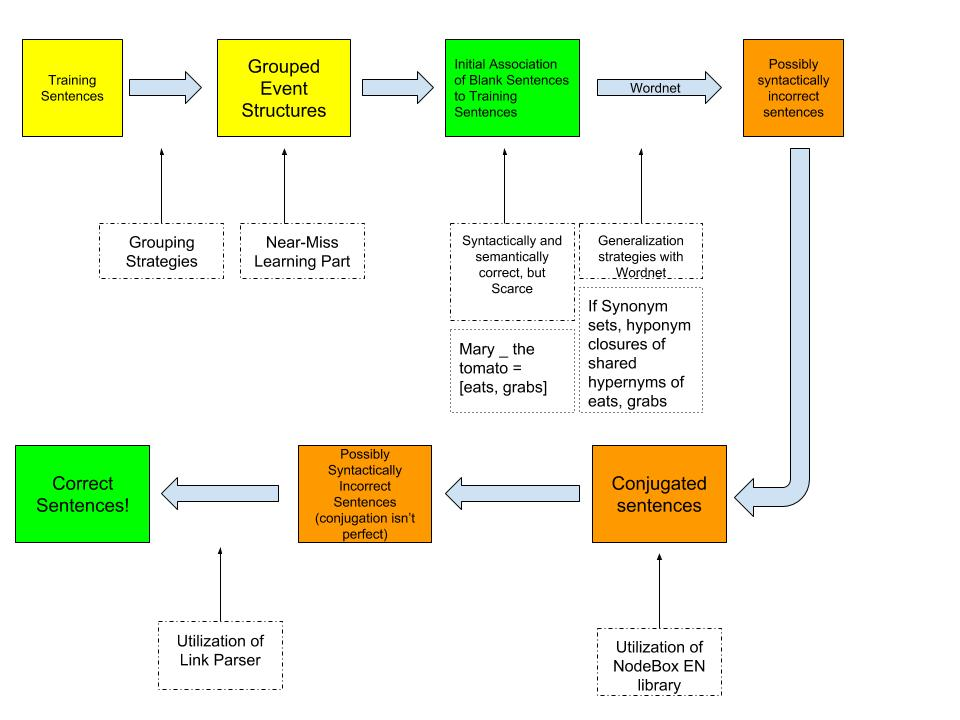
\includegraphics[width=\linewidth]{6_863_Pipeline.jpg}
  \caption{The flowchart of our computational pipeline.}
  \label{fig:boat1}
\end{figure}

\subsection{Predicting the missing word}

Our goal is to take a sentence with a missing word, such as \emph{``Mary ate the **blank**."} and replace the **blank** with a \emph{reasonable} replacement word. This task is one that people do everyday without realizing it, especially in a noisy setting or when speaking to someone with a thick accent, in order to interpret what has been said. \\

However, this task goes beyond just syntactic validity, since few people would guess that the sentence was \emph{``Mary ate a laptop".} We need to inject some notion of semantics. However, we cannot just naively apply methods from WordNet, because we are missing the word that fits in the blank. Most WordNet methods are ways of mapping from one word to other words that are related in a particular way, e.g. hypernymy or synonymy. \\

So in order to move forward, we should first come up with a way of distinguishing valid sentences in a way that lets us generate a missing word. We decided to adopt a model of \emph{language learning} that is very similar to the notion of \textbf{Near-Miss Learning} that was covered in MIT's Artificial Intelligence class 6.034. \\

Accordingly, we took a set of training sentences, used and re-factored software from Lab 3 to decompose these training sentence into their respective event structures, and grouped event structures together in a way that generalized semantically valid sentences. Here, this means \textbf{we assumed that the training corpus is semantically valid}, which is a realistic assumption (it would be irrational to train with incorrect data). \\

Below, we discuss our experimentation with different grouping and generalization strategies, in order to determine semantically valid replacements for a missing word.

However, first and foremost it is important to provide a clear definition of what \textbf{event structures} are and how they were represented in our pipeline. 

\subsubsection{Event Structures}

For any given sentence, the event structure maps the relevant "agent", "action", "tense" and "patient" fields to words/phrases within the sentence. 

For example, for the sentence ``Mary ate the tomato'', the event structure is given by \{{`action': `eat', `patient': `tomato', `tense': `past', `agent': `Mary'}…\}



\subsection{Learning from the Training Set: Strategies}

For each of the grouping strategies below, we utilized the following training set. 

Training set: 

\begin{itemize}
  \item John ate the potato.
  \item John ate the tomato.
  \item Mary ate the tomato.
\end{itemize}

As simple as it seems, this training set provided fruitful grounds for exploring these grouping strategies and coming up with generalizations. \\

It is extremely important to note that at the end, we passed more comprehensive training sets to the system. We discuss such training sets and explorations in Section 3. 

\subsubsection{No Grouping: Simplest Strategy}

This strategy simply provides a list of separate event structures of the 3 sentences in the training set: 

\begin{itemize}
\item\{{'action': 'eat', 'patient': 'potato', 'tense': 'past', 'agent': 'John'}\}
\item\{{'action': 'eat', 'patient': 'tomato', 'tense': 'past', 'agent': 'John'}\}
\item\{{'action': 'eat', 'patient': 'tomato', 'tense': 'past', 'agent': 'Mary'}\}
\end{itemize}

Hence, as the name implies, no grouping or merging of the individual event structure occurs with the No Grouping Strategy.

\subsubsection{One Difference Groupings}

This is where we initialize the notion of \textbf{near-miss learning}. 

Here, if two training sentences have the same event structure, but differ across on only one feature, we group together the values of that specific feature. This is a very conservative form of grouping. 

Below is an illustration of One Difference Grouping. 

\begin{spverbatim}
[{'action': set(['eat']), 'tense': set(['past']), 'patient': set(['tomato']), 'agent': set(['John', 'Mary'])}, {'action': set(['eat']), 'patient': set(['tomato', 'potato']), 'tense': set(['past']), 'agent': set(['John'])}]
\end{spverbatim}

The training sentences' were grouped into two. The first group is constructed by the 2 sentences ``John ate the tomato." and ``Mary ate the tomato." because differ by only one field, which is the ``agent'' field. The second group is constructed by the 2 sentences ``John ate the tomato." and ``John ate the potato."

For illustration purposes, we explore an additional grouping option: 


\subsubsection{Two Difference Groupings}

To allow more flexibility, we allowed 2 degrees of freedom within the training set. The result of the Two Difference Grouping strategy is shown below: 


\begin{spverbatim}
[{'action': set(['eat']), 'tense': set(['past']), 'patient': set(['tomato', 'potato']), 'agent': set(['John', 'Mary'])}]
\end{spverbatim}

\subsection{Application of Grouping Information to Produce Valid Candidate Sentences}

The next step in the pipeline is to leverage the information The \emph{Grouping} stage gathers. Using the grouping information, we would like to associate the missing word to possible words in the training set. 

For example, for the sentence ``Mary ate the **blank**'' we would like to list the words ``potato'' and ``tomato'' as possible fillers solely using our training set. 

For each word in the lexicon, and for each event grouping strategy the system temporarily fills in the sentence and cross-checks to find whether sentence is valid. 

For the above-mentioned training set, \textbf{this stage output potato and tomato as valid fillers} for the sentence ``Mary ate the **blank**''

This output, albeit completely valid, is scarce. In fact, \textbf{a crucial thing to do was to expand beyond the training set to understand the complexity of the problem better and reach better conclusions}.  \\

Accordingly, we leveraged WordNet to inject word-based semantics. This way, the system would be \emph{less} limited to the training set. \\ 

\subsection{Expansion With WordNet}

WordNet functionalities are extremely useful. For the sentence 
``Mary ate the **blank**'', remember that the previous stage produced \emph{tomato} and \emph{potato} as valid fillers as learned from the training set. For each of these two words, we utilized WordNet to yield synonyms, which are shown below:

\begin{itemize}
\item  Mary ate the potato.
\item\ Mary ate the white potato.
\item\ Mary ate the spud.
\item\ Mary ate the tater.
\end{itemize}

\begin{itemize}
\item\ Mary ate the tomato.
\item\ Mary ate the love apple.
\item\ Mary ate the tomato plant.
\end{itemize}

In addition to the \textbf{synonyms}, we also explored \emph{hyponym closure of shared hypernyms}.  

One extremely important aspect is to keep in mind that the missing word was a noun. These examples are valid, however, things got broken down when the blanked word isn't a noun.

For example, for verbs, \textbf{even though the previous stage necessarily produced grammatical options from the training set, directly injecting WordNet could very well break the syntax.}

Consider the example ``Mary **blank** the tomato.''

The output of Section 2.3 yields ``ate'' as a valid filler word. However, expanding on ``ate''s synsets with WordNet produced the following results: 

\begin{itemize}
\item\ Mary eat the tomato.
\item\ Mary fee the tomato.
\item\ Mary consume the tomato.
\item\ Mary deplete the tomato.
\item\ Mary chow the tomato.
\end{itemize}

These sentences are \emph{all} syntactically invalid. 

\emph{In short, WordNet provides good results when the missing word is a noun, but generally breaks the syntax when the missing word is verb}

In the next section we describe the remedy to the case when the missing word is a verb.  

\subsection{Conjugating WordNet Injections}

Since most of the verbs yielded by WordNet would be in the base form such as eat, take, grab etc. , \textbf{we wrote our own verb conjugator to conjugate the base form verbs leveraging information from the event structures learnt from the training set and NodeBox English Linguistics library. }

An example conjugation is shown below: 

\begin{itemize}
\item\ Mary eats the tomato.
\item\ Mary fees the tomato.
\item\ Mary consumes the tomato.
\item\ Mary depletes the tomato.
\item\ Mary chows the tomato.
\end{itemize}

\subsection{Further Syntax-Checking Conjugated Sentences}

To further enforce accuracy, we passed the conjugated verbs through Carnegie Mellon University's Link Parser -See 10. 

Since this is the last stage in the pipeline, we report the correct sentences in the next section, discuss and provide further extensions to the results. 

\section{Results}

Following the description of our methodology, let's continue with results coming from the following 3 examples. 
\begin{enumerate}
\item\ **blank** ate the tomato.
\item\ Mary **blank** the tomato.
\item\ Mary ate the **blank**. 
\end{enumerate}

It isn't hard to see that these 3 examples come from the same sentence, but \emph{different parts taken off.}

For 1, **blank** ate the tomato,  the pipeline's output included the sentences below. For the full output list, please see 11. 

\begin{itemize}
\item\ Mary ate the tomato
\item\ Virgin Mary ate the tomato
\item\ The Virgin ate the tomato
\item\ Blessed Virgin ate the tomato
\item\ Madonna ate the tomato
\item\ John ate the tomato
\item\ Mary ate the tomato
\item\ John ate the tomato
\item\ King John ate the tomato
\item\ Saint John ate the tomato
\item\ Saint John the Apostle ate the tomato
\item\ John the Evangelist ate the tomato
\item\ John the Divine ate the tomato
\item\ Gospel According to John ate the tomato
\end{itemize}


For 2, Mary **blank** the tomato, the pipeline's output included the sentences below: 

\begin{itemize}
\item\ Mary eats the tomato.
\item\ Mary fees the tomato.
\item\ Mary consumes the tomato.
\item\ Mary depletes the tomato.
\item\ Mary chows the tomato.
\end{itemize}

For 3, Mary ate the **blank**, the pipeline's output included the sentences below: 

\begin{itemize}
\item\ Mary ate the tomato.
\item\ Mary ate the tomato.
\item\ Mary ate the potato.
\item\ Mary ate the white potato.
\item\ Mary ate the Irish potato.
\item\ Mary ate the murphy.
\item\ Mary ate the spud.
\item\ Mary ate the tater.
\item\ Mary ate the potato.
\item\ Mary ate the white potato.
\item\ Mary ate the white potato vine.
\item\ Mary ate the Solanum tuberosum.
\item\ Mary ate the tomato.
\item\ Mary ate the tomato.
\item\ Mary ate the love apple.
\item\ Mary ate the tomato plant.
\item\ Mary ate the Lycopersicon esculentum.
\item\ Mary ate the potato.
\item\ Mary ate the tomato.
\end{itemize}

These sentences are all syntactically and semantically valid. Now, \emph{one can easily see 2 distinct yet exciting paths to follow: \textbf{further expand or further generalize}} \\

\subsection{Further Generalizing from Results}
We first start with generalizations. An extremely tempting step to take is to find rules of generalization in our training set. For example, what if we noticed that there was something in common to many of the suggestions, whether they be tomato or potato? Fundamentally, "Mary ate the **blank**" should semantically match any food item.

Following this idea, we explored a generalization pattern by shared hypernymy. The core idea is to find shared hypernyms between the \emph{very initial guesses given by the near-miss learning stage}. 

Consider the example below: 

Passing in ``Mary ate the **blank**" produces tomato and potato at the near-miss learning stage. Looking at the shared hypernyms of tomato and potato, one sees: 

\begin{enumerate}
\item\ vascular plant
\item\ tracheophyte
\end{enumerate}

As simple as it seems, this sheds promising light. In addition to the generalization, this information provides valuable insight into the training set. 

\subsubsection{Further Expand From Results}

Another path to take from the results is to further expand the possibilities. We explored the idea by taking the transitive closure of hyponymy under these objects. 

Some of the results of expansion are shown below. Since the list is very long, we only reported a small fraction below. For the full list of results, please see 11.

\begin{verbatim}
[u'aquatic_plant', u'water_plant', u'hydrophyte', u'hydrophytic_plant',
u'bulbous_plant', u'cormous_plant', u'creeper', u'cultivar', 
u'cultivated_plant', u'deciduous_plant', u'desert_plant', u'xerophyte', 
u'xerophytic_plant', u'xerophile', u'xerophilous_plant', u'evergreen', 
u'evergreen_plant', u'geophyte', u'halophyte', u'herb', u'herbaceous_plant', 
u'mesophyte', u'mesophytic_plant', u'psilophyte', u'psilophyton', 
u'pteridophyte', u'nonflowering_plant', u'spermatophyte', u'phanerogam', 
u'seed_plant', u'succulent', u'tuberous_plant', u'vine', u'weed', 
u'woody_plant', u'ligneous_plant', u'American_frogbit', u'Limnodium_spongium',
u'arrow_arum', u'awlwort', u'Subularia_aquatica', u'cryptocoryne', 
u'water_trumpet', u'duckweed', u'eelgras', u'grass_wrack', u'sea_wrack', 
u'Zostera_marina', u'featherfoil', u'feather-foil', u'frogbit', u"frog's-bit",
u'Hydrocharis_morsus-rana', u'golden_club', u'Orontium_aquaticum', 
u'golden_saxifrage']


\end{verbatim}

\section{Discussion and Future Work}

Through a comprehensive computational pipeline we explored the seemingly easy, yet inherently complex problem of Filling in the Gap. 

We were able to create a pipeline that, given the particular sentence structure of \textbf{agent, action, patient} \emph{or} \textbf{agent, action} can fill in the gaps accurately while maintaining the syntax and semantics. One limitation of the system was that the blanked out word had to be either a noun (proper or regular) or a verb. Support for additional parts of speech is possible, which we discuss in the Future Work section. 

Importantly, we saw that solutions to the Fill In The Gap problem could very well provide a path to the \textbf{generalization to the training corpus} as well as \textbf{expansion from the training corpus}. 

\subsection{Future Work}

Throughout the project we explored countless language tools, and saw how hard and complex Filling In The Gap problem is and found multiple, pivotal areas that can be further explored or simply added to our solution. 

First of all, support for additional sentence structures such as question phrases may be added. \\

Second, support for additional parts of speech may be added to support adjectives, for instance. Currently, as we mentioned, our pipeline only produces valid results when the removed word is a noun or a verb. Verbs are arguably the most complex parts of a sentence. Hence, adding support for adjectives is a fairly realistic improvement after having done verbs. \\

Third, currently the grouping stage takes the entire information from the training corpus. It would be an interesting area of research to consider injecting WordNet synsets during the information acquisition stage of grouping. \\

Finally, and most importantly, currently the way our system handles grouping is greedy. One thing to consider would be to add a grouping procedure that only groups according to the N/log(N) human learning rule as we covered in lecture. 


\section{Conclusion and Remarks on Fill In The Gaps Problem}

We sought to tackle the filling in the gaps problem using the theory and experience we got from 6.863. The problem, as was initially mentioned, required 3 parts each of which pertained to a specific assignment we did in the class. When filling in a word, the sentence must preserve its syntax. Next, the sentence needs to preserve the `meaning' aspect which composes to sentence and word semantics. Using syntactic and semantic parsers and WordNet, we heavily extended on our class assignments to engineer a computational pipeline that, given a particular sentence structure and a particular type of missing word, learns from a training corpus and generates valid sentences filled in with candidate words. 

Throughout, this process showed us that it was indeed possible to tackle the fill in the gaps problem. We saw that while solving the problem we could also learn generalization information from the training data. Most importantly, we saw that Fill In The Gaps problem is inherently modular and complex. It is complex because it needs to be tamed with syntax and semantics. It is modular because our pipeline solved the problem for different word types.    

\newpage
\section{References}

\begin{spverbatim}
[1] S. Bird, E. Loper, and E. Klein. NLTK 3.2.5 Documentation. https://www.nltk.org/
[2] G. Miller, R. Beckwith, C. Fellbaum, D. Gross, and K. Miller. 
    Introduction to WordNet: An On-Line Lexical Database. 1993. 
    http://wordnetcode.princeton.edu/5papers.pdf 
[3] ccg2lambda: Composing Semantic Representations Guided by CCG Derivations. 
    https://github.com/mynlp/ccg2lambda
[4] The Penn Treebank: An Overview
https://pdfs.semanticscholar.org/182c/4a4074e8577c7ba5cbbc52249e41270c8d64.pdf
[5] Feature Grammar Parsing. http://www.nltk.org/howto/featgram.html
[6] S. Bird, E. Loper, and E. Klein. Building Feature Based Grammars. 
    2014. http://www.nltk.org/book/ch09.html
[7] T. Mikolov, I. Sutskever, K. Chen, G. Corrado, J. Dean. 
    Distributed Representations of Words and Phrases and their Compositionality. 
    2013. https://papers.nips.cc/paper/5021-distributed-representations
    -of-words-and-phrases-and-their-compositionality.pdf 
[8] M. Marcus, B. Santorini, M. Marcinkiewicz, and A. Taylor. Penn Treebank Sample. 
    Philadelphia: Linguistic Data Consortium. 1999. https://catalog.ldc.upenn.edu/ldc99t42
[9] S. Bird, E. Loper, and E. Klein. Source Code for nltk.grammar. 
    2017. http://www.nltk.org/_modules/nltk/grammar.html
[10] D. Temperley, D. Sleator, and J. Lafferty. Source code for Link Grammar. 
http://www.link.cs.cmu.edu/link/
[11] S. Viteri, M. Savran, and W. Mitchell. 6.863 Final Project.
https://github.com/scottviteri/6.863FinalProject
\end{spverbatim}

\end{document}


